\section{Model SV2TTS}
Model Speech Vector to TTS (SV2TTS) terdiri dari tiga bagian, masing-masing dilatih secara individual.
Hal ini memungkinkan setiap bagian dilatih pada data independen, sehingga mengurangi kebutuhan untuk mendapatkan data multispeaker berkualitas tinggi.

\begin{figure}[H]
        \centerline{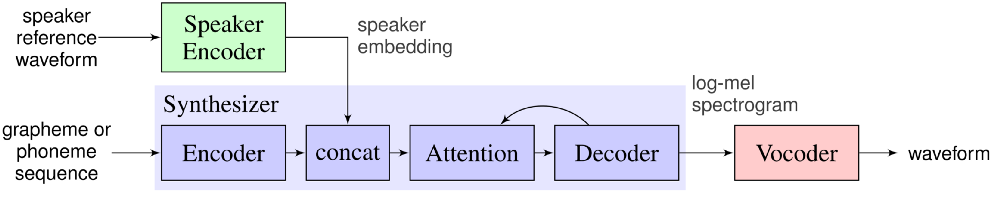
\includegraphics[scale=.35]{figures/arsitektur}}
        \caption{Arsitektur SV2TTS umum Sumber: Jia, Zhang, dan Weiss et al.}
		\label{arsitektur}
\end{figure}

\subsection{Speaker Encoder}

Bagian pertama dari model SV2TTS adalah encoder speaker.
Tugas speaker encoder adalah mengambil beberapa input audio (dikodekan sebagai bingkai spektogram mel), dari speaker tertentu, dan mengeluarkan embedding yang menangkap "bagaimana suara speaker". Encoder pembicara tidak peduli dengan kata-kata yang diucapkan pembicara, atau tentang kebisingan di latar belakang, yang dia pedulikan hanyalah suara pembicara, misalnya, suara bernada tinggi/rendah, aksen, nada, dll. Semua fitur ini digabungkan menjadi vektor berdimensi rendah, yang secara formal dikenal sebagai vektor-d, atau secara informal sebagai penyematan speaker. Akibatnya, ujaran yang diucapkan oleh penutur yang sama akan saling berdekatan pada penyematan penutur, sedangkan tuturan yang diucapkan oleh penutur yang berbeda akan berjauhan pada penyematan penutur.
\begin{figure}[H]
        \centerline{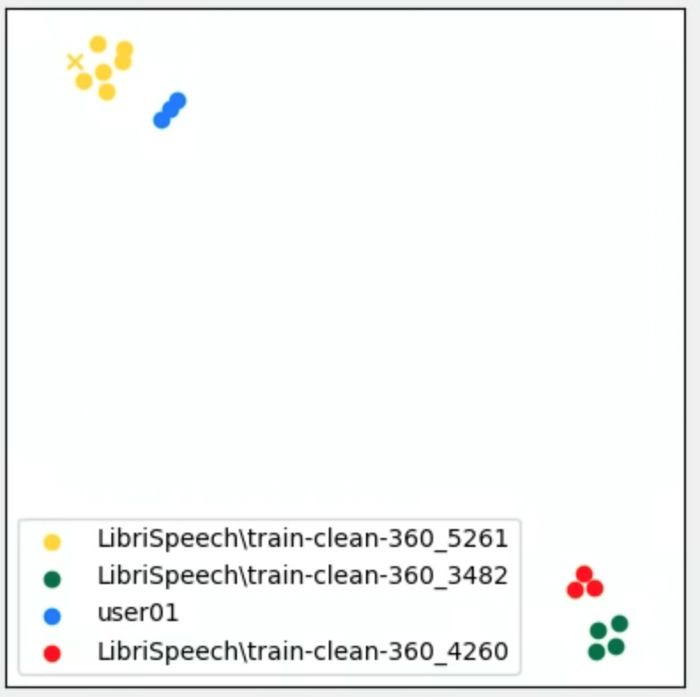
\includegraphics[scale=.35]{figures/encoder}}
        \caption{Representasi visual dari embeddings, setiap warna adalah speaker yang berbeda Sumber: Jia, Zhang, dan Weiss et al.}
		\label{encoder}
\end{figure}

Untuk belajar menghasilkan embeddings ini, penulis menjelaskan proses berikut:
\begin{enumerate}
\item Pertama, contoh audio ucapan disegmentasi menjadi klip 1,6 detik tanpa transkrip dan diubah menjadi spektogram mel.
\item Kemudian speaker encoder dilatih untuk mengambil dua sampel audio dan memutuskan apakah speaker yang sama memproduksinya atau tidak. Sebagai produk sampingan, ini memaksa encoder speaker untuk membuat embeddings yang mewakili suara speaker.
\end{enumerate}
Proses pelatihan mirip dengan jaringan saraf siam jika Anda sudah familiar dengan mereka.

\subsection{Synthesizer}
Synthesizer adalah bagian dari SV2TTS yang menganalisis input teks untuk membuat spektogram mel, yang kemudian diubah oleh vocoder menjadi suara.
Synthesizer mengambil urutan teks — dipetakan ke fonem (unit terkecil dari suara manusia, misalnya, suara yang Anda buat saat mengucapkan 'a'), bersama dengan embeddings yang dihasilkan oleh encoder speaker, dan menggunakan arsitektur Tacotron 2 untuk menghasilkan bingkai dari spektogram mel secara berulang
\begin{figure}[H]
        \centerline{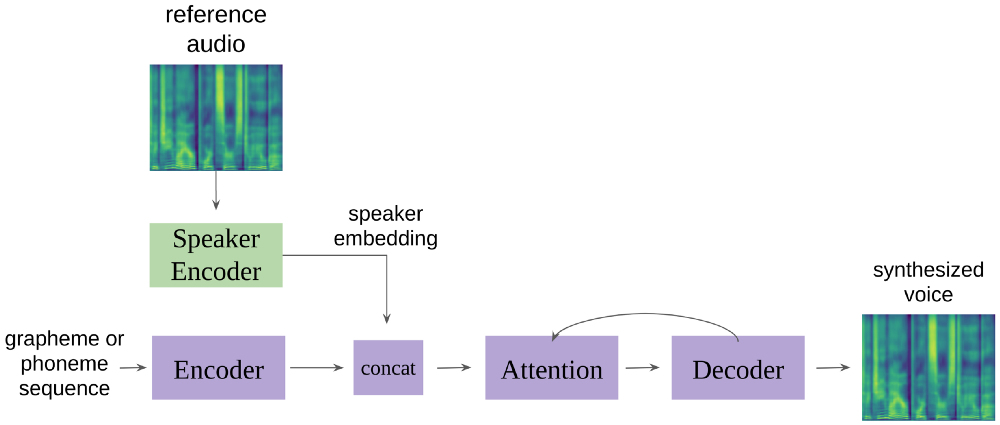
\includegraphics[scale=.35]{figures/model}}
        \caption{Model Arsitektur Multi-Speaker Voice Cloning Sumber: Jia, Zhang, dan Weiss et al.}
		\label{model}
\end{figure}

Berikut Proses Training Synthesizer:

\begin{enumerate}
\item Pertama, kami mengumpulkan urutan fonem dan spektogram mel dari pembicara yang mengucapkan kalimat itu.
\item Kemudian, spektogram mel diteruskan ke encoder speaker untuk menghasilkan embedding speaker.
\item Selanjutnya, pembuat enkode penyintesis menggabungkan penyandian urutan fonemnya dengan penyematan speaker.
\item Spektogram mel dihasilkan secara berulang oleh decoder dan bagian perhatian dari synthesizer
\item Terakhir, spektogram mel dibandingkan dengan target awal untuk menghasilkan kerugian, yang kemudian dioptimalkan
\end{enumerate}

\begin{figure}[H]
        \centerline{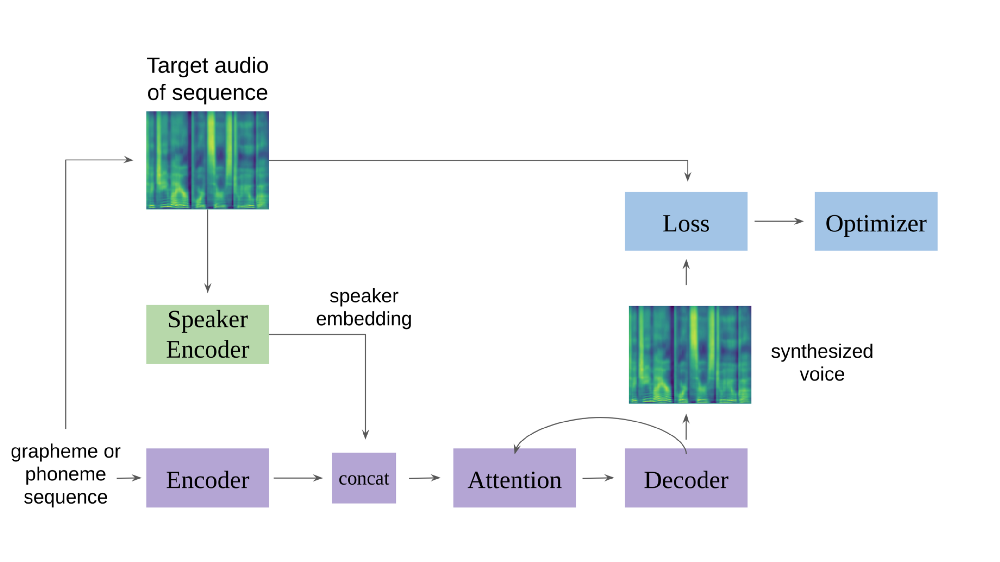
\includegraphics[scale=.35]{figures/train}}
        \caption{Training Synthesizer Sumber: Jia, Zhang, dan Weiss et al.}
		\label{train}
\end{figure}

\subsection{Vocoder}
Pada titik ini, synthesizer telah membuat spektogram mel, tetapi kami masih belum dapat mendengarkan apa pun. Untuk mengubah spektogram mel menjadi gelombang audio mentah, penulis menggunakan vocoder.
Vocoder khusus yang digunakan di sini didasarkan pada model WaveNet DeepMind , yang menghasilkan bentuk gelombang audio mentah dari teks, dan pada satu titik canggih untuk sistem TTS.
\begin{figure}[H]
        \centerline{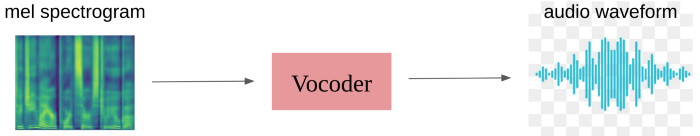
\includegraphics[scale=.35]{figures/vocoder}}
        \caption{Vocoder Sumber: Jia, Zhang, dan Weiss et al.}
		\label{vocoder}
\end{figure}


\subsection{Alur Model SV2TTS}
berikut adalah alur modelnya:
\begin{enumerate}
\item Encoder speaker mendengarkan sampel audio yang diberikan dan menghasilkan embedding
\item Synthesizer mengambil daftar fonem dan penyematan speaker, kemudian menghasilkan spektogram mel
\item Vocoder saraf menguraikan spektogram mel menjadi bentuk gelombang audio yang dapat kita dengarkan
\end{enumerate}

\subsection{Mengukur Kualitas Hasil}
Penulis menggunakan penilai manusia untuk mengukur kealamian dan kesamaan ucapan yang dihasilkan model.
Kealamian mengukur seberapa "manusia" ucapan itu terdengar, sementara kesamaan mengukur seberapa mirip suara pidato yang disintesis dengan pembicara aslinya.
Penilai berinteraksi melalui GUI yang terlihat seperti:
\begin{figure}[H]
        \centerline{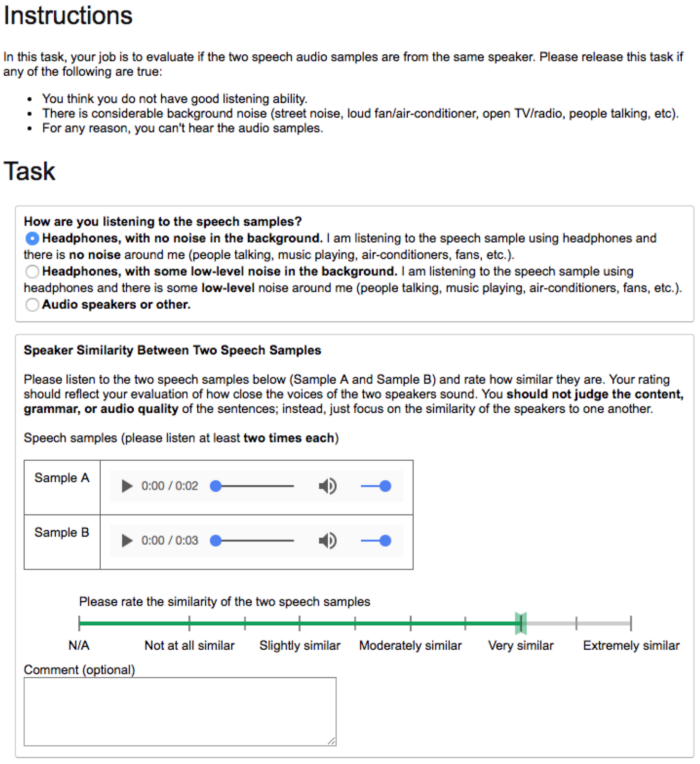
\includegraphics[scale=.45]{figures/nilai}}
        \caption{Pengukuran Kualitas Model Sumber: Jia, Zhang, dan Weiss et al.}
		\label{nilai}
\end{figure}
Teknik penggunaan rating crowdsourced seperti ini sering disebut dengan Mean Opinion Score atau MOS.
Penulis menemukan bahwa hasil akhir untuk kealamian akhirnya terlihat seperti:
\begin{figure}[H]
        \centerline{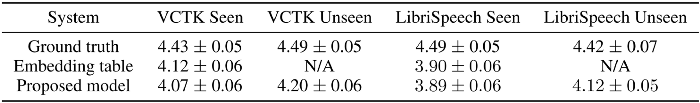
\includegraphics[scale=.45]{figures/hasil}}
        \caption{MOS Sumber: Jia, Zhang, dan Weiss et al.}
		\label{mos}
\end{figure}

Jika Anda ingin analisis lengkap ini, saya akan merekomendasikan membaca bagian 3.1 dari makalah asli. Namun, secara ringkas:
\begin{enumerate}
\item Model SV2TTS yang diusulkan mencapai sekitar 4,0 MOS di semua kumpulan data.
\item LibriSpeech (salah satu set data pelatihan) diklasifikasikan sebagai kurang alami, karena tidak ada tanda baca dalam transkrip, sehingga menyulitkan model untuk mempelajari jeda.
\item Sistem tabel penyematan menggunakan tabel pencarian penyematan speaker tetapi sebaliknya memiliki arsitektur yang sama. \item Karena memiliki tabel pencarian, tidak dapat digeneralisasi, dan oleh karena itu tidak dapat dievaluasi pada kumpulan data yang tidak terlihat.
\item Kealamian dari contoh yang tidak terlihat dan yang terlihat sangat mirip, yang sangat mengesankan.
\end{enumerate}
Dan untuk kesamaan ucapan, hasilnya terlihat seperti:
\begin{figure}[H]
        \centerline{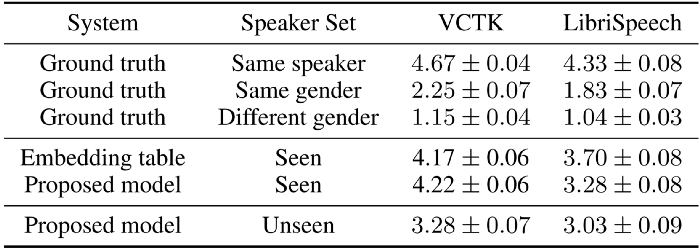
\includegraphics[scale=.35]{figures/hasil1}}
        \caption{Speech Similarity Sumber: Jia, Zhang, dan Weiss et al.}
		\label{similar}
\end{figure}
Sekali lagi, Anda mungkin ingin membaca bagian 3.2 dari makalah asli untuk analisis lengkapnya. Tapi secara ringkas:
\begin{enumerate}
\item Skor lebih tinggi untuk VCTK (set data pelatihan lainnya), menunjukkan bentuk dataset yang lebih terstruktur.
\item Skor model SV2TTS antara "cukup mirip" dan "sangat mirip" pada skala evaluasi untuk pembicara yang tidak terlihat.
\item Meskipun ini sulit diukur secara matematis, model secara keseluruhan menangkap karakteristik pembicara secara akurat.
\end{enumerate}